% FSB Seminar — Sveučilište u Zagrebu, Fakultet strojarstva i brodogradnje
% Template v2.1 — latex_architect popunjava placeholdere iz project.yaml

\documentclass[12pt,a4paper]{article}

% --- Encoding, Font & Language (dual-engine) ---
% Kanonski engine je Tectonic (XeTeX): fontspec + TeX Gyre Termes ima PRAVI
% OpenType bold pa hrvatski ž/ć/š/đ rade i u \textbf{}. pdfLaTeX fallback koristi
% newtxtext (vidi gotcha miktex-t1-bold-diacritics). NE newtxmath uz amssymb (\Bbbk konflikt).
\usepackage{iftex}
\ifPDFTeX
  \usepackage[utf8]{inputenc}
  \usepackage[T1]{fontenc}
  \usepackage{newtxtext}
\else
  \usepackage{fontspec}
  \setmainfont{texgyretermes-regular.otf}[
    BoldFont       = texgyretermes-bold.otf,
    ItalicFont     = texgyretermes-italic.otf,
    BoldItalicFont = texgyretermes-bolditalic.otf
  ]
\fi
\usepackage[croatian]{babel}

% --- Layout ---
\usepackage[top=2.5cm,bottom=2.5cm,left=2.5cm,right=2.5cm]{geometry}
\usepackage{setspace}
\usepackage{microtype}
\onehalfspacing

% --- Headers & Footers ---
\usepackage{fancyhdr}
\setlength{\headheight}{16.5pt}
\pagestyle{fancy}
\fancyhf{}
\renewcommand{\sectionmark}[1]{\markboth{\thesection.\ #1}{}}
\fancyhead[L]{\small\itshape\nouppercase{\leftmark}}
\fancyhead[R]{\small\itshape \seminartitleshort}
\fancyfoot[L]{\small\itshape Krešimir Hartl — Fakultet strojarstva i brodogradnje}
\fancyfoot[R]{\small\itshape\thepage}
\renewcommand{\headrulewidth}{0.4pt}
\renewcommand{\footrulewidth}{0.4pt}

% --- Section Formatting (14pt Bold Uppercase) ---
\usepackage{titlesec}
\titleformat{\section}
  {\normalfont\fontsize{14}{17}\bfseries\MakeUppercase}
  {\thesection.}{0.5em}{}
\titleformat{\subsection}
  {\normalfont\fontsize{12}{15}\bfseries}
  {\thesubsection.}{0.5em}{}
\titleformat{\subsubsection}
  {\normalfont\fontsize{12}{15}\bfseries\itshape}
  {\thesubsubsection.}{0.5em}{}
\titleformat{\paragraph}[runin]
  {\normalfont\fontsize{12}{15}\itshape}
  {}{0em}{}[.]

% Svako poglavlje (\section) pocinje na novoj stranici.
\newcommand{\sectionbreak}{\clearpage}

% --- Figures & Tables ---
\usepackage{graphicx}
\usepackage{booktabs}
\usepackage{tabularx}
\usepackage{longtable}
\usepackage{array}
\usepackage{float}
\usepackage{caption}
\captionsetup[figure]{font={small,bf},labelsep=period,position=below}
\captionsetup[table]{font={small,bf},labelsep=period,position=above}

% --- Figure/Table numbering by section (Slika 2.1, Tablica 2.1) ---
\usepackage{chngcntr}
\counterwithin{figure}{section}
\counterwithin{table}{section}
\counterwithin{equation}{section}

% --- Depth ---
\setcounter{secnumdepth}{3}
\setcounter{tocdepth}{3}

% --- Croatian names (addto — babel croatian overrida renewcommand) ---
\addto\captionscroatian{%
  \renewcommand{\figurename}{Slika}%
  \renewcommand{\tablename}{Tablica}%
  \renewcommand{\contentsname}{\normalfont\fontsize{14}{17}\bfseries SADRŽAJ}%
  \renewcommand{\listfigurename}{\normalfont\fontsize{14}{17}\bfseries POPIS SLIKA}%
  \renewcommand{\listtablename}{\normalfont\fontsize{14}{17}\bfseries POPIS TABLICA}%
  \renewcommand{\refname}{\normalfont\fontsize{14}{17}\bfseries LITERATURA}%
}

% --- References ---
\usepackage{cite}
\usepackage{etoolbox}
% Bibliografska jedinica ne smije ostati rascijepljena između dviju stranica.
\AtBeginEnvironment{thebibliography}{\interlinepenalty=10000}

% --- Umetanje vanjskih PDF stranica (sken zadatka) ---
\usepackage{pdfpages}

% --- Hyperlinks ---
\usepackage[hidelinks,unicode]{hyperref}

% --- Math ---
\usepackage{amsmath}
\usepackage{amssymb}

% --- Color ---
\usepackage{xcolor}

% --- MATLAB kod i ispis rjesavaca ---
\usepackage{listings}
\lstdefinestyle{matlabstyle}{
  language=Matlab,
  basicstyle=\ttfamily\footnotesize,
  keywordstyle=\bfseries,
  commentstyle=\itshape,
  stringstyle=\normalfont,
  numbers=none,
  frame=single,
  framesep=4pt,
  rulecolor=\color{black!45},
  breaklines=true,
  breakatwhitespace=false,
  columns=fullflexible,
  keepspaces=true,
  showstringspaces=false,
  tabsize=2,
  aboveskip=8pt,
  belowskip=8pt,
  extendedchars=true,
  literate={č}{{\v c}}1 {ć}{{\'c}}1 {ž}{{\v z}}1 {š}{{\v s}}1 {đ}{{\dj}}1
           {Č}{{\v C}}1 {Ć}{{\'C}}1 {Ž}{{\v Z}}1 {Š}{{\v S}}1 {Đ}{{\DJ}}1
}
\lstdefinestyle{outputstyle}{
  basicstyle=\ttfamily\footnotesize,
  keywordstyle=\normalfont,
  commentstyle=\normalfont,
  numbers=none,
  frame=single,
  framesep=4pt,
  rulecolor=\color{black!25},
  backgroundcolor=\color{black!4},
  breaklines=true,
  columns=fullflexible,
  keepspaces=true,
  showstringspaces=false,
  aboveskip=8pt,
  belowskip=8pt,
}
\lstset{style=matlabstyle}
\renewcommand{\lstlistingname}{Ispis}

% --- Paragraph spacing ---
\setlength{\parindent}{1.25cm}
\setlength{\parskip}{0pt}

% --- Stabilan prijelom teksta, formula i referenci ---
% Bez hifenacije; microtype i umjereni emergency stretch čuvaju poravnanje
% bez velikih međurječnih praznina i bez overfull redaka.
\hyphenpenalty=10000
\exhyphenpenalty=10000
\binoppenalty=10000
\relpenalty=10000
\clubpenalty=10000
\widowpenalty=10000
\displaywidowpenalty=10000
\brokenpenalty=10000
\tolerance=3000
\hbadness=10000
\emergencystretch=2em

% ============================================================
% DOCUMENT METADATA — latex_architect popunjava iz project.yaml
% ============================================================
\newcommand{\univname}{SVEUČILIŠTE U ZAGREBU}
\newcommand{\facultyname}{FAKULTET STROJARSTVA I BRODOGRADNJE}
\newcommand{\coursename}{OPTIMIZACIJSKE METODE U RAZVOJU I UPRAVLJANJU SUSTAVA}
\newcommand{\seminartitle}{Optimizacijske metode u razvoju i upravljanju sustava}
\newcommand{\seminartitleshort}{OMuRiUS — Seminarski rad}
\newcommand{\professorname}{Prof. dr. sc. Andrej Jokić}
\newcommand{\authorname}{Krešimir Hartl}
\newcommand{\locationdate}{Zagreb, 2026.}
% Sken izvornog teksta zadatka, umece se odmah iza naslovnice.
\newcommand{\taskscan}{zadatak/zadatak_sken.pdf}

% ============================================================
\begin{document}

% Sken zadatka je PDF 1.7; izlazna verzija mora biti barem tolika.
\ifPDFTeX\else\special{pdf:minorversion 7}\fi

% ---- TITLE PAGE ----
\begin{titlepage}
  \centering
  {\fontsize{14}{17}\selectfont \univname \par}
  {\fontsize{14}{17}\selectfont \facultyname \par}
  \vfill
  {\fontsize{20}{26}\bfseries SEMINARSKI RAD \par}
  \vspace{0.8cm}
  {\fontsize{18}{24}\bfseries \coursename \par}
  \vfill
  % Tabular: lijevo "Profesor:" / bold ime — desno "Student:" / bold ime
  \begin{tabular}{p{0.45\textwidth}>{\raggedleft\arraybackslash}p{0.45\textwidth}}
    \textmd{Profesor:} & \textmd{Student:} \\[0.3cm]
    \textbf{\professorname} & \textbf{\authorname}
  \end{tabular}
  \vspace{1.5cm}
  \par
  {\normalfont \locationdate \par}
\end{titlepage}

% ---- FRONTMATTER (rimske stranice velikim slovima: I, II, III) ----
\pagenumbering{Roman}
\setcounter{page}{1}

% ---- IZVORNI TEKST ZADATKA (sken, bez zaglavlja i paginacije) ----
% pageanchor=false: umetnute stranice ne smiju stvarati hyperref sidra.
\hypersetup{pageanchor=false}
\includepdf[pages=-,fitpaper=true,pagecommand={\thispagestyle{empty}}]{\taskscan}
\hypersetup{pageanchor=true}

\tableofcontents
\clearpage

% ---- BODY (arapske stranice) ----
\pagenumbering{arabic}
\setcounter{page}{1}

\section{Uvod}

U ovom seminarskom radu rješavaju se četiri zadatka iz kolegija \textit{Optimizacijske metode u razvoju i upravljanju sustava}. Redom su to: kvadratni program s dva ograničenja nejednakosti, njegova robusna inačica uz intervalnu nesigurnost koeficijenata, formulacija nivelacije uzdužnog profila ceste kao linearnog programa te sinteza regulatora po varijablama stanja za sklopni linearni sustav pomoću linearnih matričnih nejednakosti.

Zajednička nit svih zadataka je konveksnost: nakon što se problem zapiše u standardnom obliku (LP, QP ili SDP), lokalni optimum je ujedno globalan, a KKT uvjeti odnosno linearne matrične nejednakosti daju provjerljiv certifikat optimalnosti ili stabilnosti~\cite{boyd2004convex,jokic2024predavanja}.

Svi proračuni provedeni su u MATLAB-u (verzija R2025b): \texttt{quadprog} za kvadratne programe u zadacima 1 i 2, \texttt{linprog} za linearni program u zadatku 3 te YALMIP sa rješavačem SDPT3 za semidefinitni program u zadatku 4. Skripte se nalaze u prilogu; svaka brojka i svaka slika u radu proizlazi iz jednog pokretanja tih skripti.

Poglavlja slijede numeraciju zadataka:
\begin{itemize}
    \item \textbf{Poglavlje 2} --- Zadatak 1: konveksnost, KKT uvjeti, \texttt{quadprog}, Lagrangeov dualni problem i osjetljivost optimalne vrijednosti.
    \item \textbf{Poglavlje 3} --- Zadatak 2: robusni ekvivalent uz nesigurnost koeficijenata od $\pm 15\%$ i usporedba s nominalnim rješenjem.
    \item \textbf{Poglavlje 4} --- Zadatak 3: diskretizacija konačnim razlikama, LP formulacija i rješenja za četiri zadana slučaja.
    \item \textbf{Poglavlje 5} --- Zadatak 4: stabilnost pojedinih modova, simulacija sklopnog sustava i LMI sinteza stabilizirajućeg regulatora.
\end{itemize}

\section{Kvadratno programiranje, KKT uvjeti, dualnost i analiza osjetljivosti}

\subsection{Opis problema i provjera konveksnosti}

Zadan je optimizacijski problem kvadratnog programiranja (engl. \textit{Quadratic Programming} -- QP) s dvije projektne varijable $x = [x_1, x_2]^T \in \mathbb{R}^2$ i dva ograničenja nejednakosti:
\begin{equation}
\min_{x \in \mathbb{R}^2} \quad f(x) = x_1^2 + 2x_2^2 - 0.3 x_1 x_2 + 2x_1 - 3x_2
\label{eq:qp_primal}
\end{equation}
uz ograničenja:
\begin{align}
g_1(x) &= a_{11} x_1 + a_{12} x_2 + 10 \leq 0, \label{eq:qp_g1} \\
g_2(x) &= a_{21} x_1 + a_{22} x_2 - 3 \leq 0, \label{eq:qp_g2}
\end{align}
gdje su nominalne numeričke vrijednosti koeficijenata:
\begin{equation}
a_{11} = -1, \quad a_{12} = -1, \quad a_{21} = 1, \quad a_{22} = -1.
\end{equation}
Ograničenja u eksplicitnom obliku glase:
\begin{align}
g_1(x) &= -x_1 - x_2 + 10 \leq 0 \iff x_1 + x_2 \geq 10, \\
g_2(x) &= x_1 - x_2 - 3 \leq 0 \iff x_1 - x_2 \leq 3.
\end{align}

\subsubsection{Matrični kanonski zapis i dokaz stroge konveksnosti}

Funkcija cilja $f(x)$ može se prikazati u simetričnom matričnom obliku:
\begin{equation}
f(x) = \frac{1}{2} x^T Q x + c^T x,
\label{eq:qp_canonical}
\end{equation}
gdje su Hesseova matrica $Q = \nabla^2 f(x) \in \mathbb{R}^{2 \times 2}$ i vektor linearnog dijela $c \in \mathbb{R}^2$ definirani kao:
\begin{equation}
Q = \begin{bmatrix} 2 & -0.3 \\ -0.3 & 4 \end{bmatrix}, \quad c = \begin{bmatrix} 2 \\ -3 \end{bmatrix}.
\end{equation}
Uvrštavanjem se potvrđuje identitet:
\begin{equation}
\frac{1}{2} \begin{bmatrix} x_1 & x_2 \end{bmatrix} \begin{bmatrix} 2 & -0.3 \\ -0.3 & 4 \end{bmatrix} \begin{bmatrix} x_1 \\ x_2 \end{bmatrix} + \begin{bmatrix} 2 & -3 \end{bmatrix} \begin{bmatrix} x_1 \\ x_2 \end{bmatrix} = x_1^2 + 2x_2^2 - 0.3 x_1 x_2 + 2x_1 - 3x_2 \equiv f(x).
\end{equation}

Da bi funkcija cilja $f(x)$ bila strogo konveksna na čitavom prostoru $\mathbb{R}^2$, nužno je i dovoljno da je Hesseova matrica $Q$ simetrična i strogo pozitivno definitna ($Q \succ 0$). Svojstvene vrijednosti matrice $Q$ određuju se iz karakterističnog polinoma:
\begin{equation}
\det(\lambda I - Q) = \det \begin{bmatrix} \lambda - 2 & 0.3 \\ 0.3 & \lambda - 4 \end{bmatrix} = (\lambda - 2)(\lambda - 4) - 0.09 = \lambda^2 - 6\lambda + 7.91 = 0.
\end{equation}
Rješenja karakteristične jednadžbe iznose:
\begin{equation}
\lambda_{1,2} = \frac{6 \pm \sqrt{36 - 4 \cdot 7.91}}{2} = \frac{6 \pm \sqrt{4.36}}{2} \approx \frac{6 \pm 2.088061}{2},
\end{equation}
odnosno:
\begin{equation}
\lambda_1 \approx 1.955969 > 0, \quad \lambda_2 \approx 4.044031 > 0.
\end{equation}
Budući da su obje svojstvene vrijednosti strogo pozitivne ($\lambda_i > 0$), matrica $Q$ je pozitivno definitna ($Q \succ 0$), što dokazuje da je funkcija cilja $f(x)$ **strogo konveksna**~\cite{boyd2004convex}.

\subsubsection{Konveksnost dopustivog skupa i globalna optimalnost}

Dopustivi skup $\mathcal{F} \subset \mathbb{R}^2$ definiran je presjekom dva poluprostora:
\begin{equation}
\mathcal{F} = \{x \in \mathbb{R}^2 \mid g_1(x) \leq 0, \; g_2(x) \leq 0\} = \{x \in \mathbb{R}^2 \mid A x \leq b\},
\end{equation}
gdje su:
\begin{equation}
A = \begin{bmatrix} -1 & -1 \\ 1 & -1 \end{bmatrix}, \quad b = \begin{bmatrix} -10 \\ 3 \end{bmatrix}.
\end{equation}
Budući da su funkcije ograničenja $g_1(x)$ i $g_2(x)$ afine (linearne), njihovi podnivo-skupovi su zatvoreni poluprostori, a presjek proizvoljnog broja konveksnih skupova je konveksan skup. Stoga je dopustivo područje $\mathcal{F}$ konveksan poliedar. 

Budući da je funkcija cilja $f(x)$ strogo konveksna, a dopustivi skup $\mathcal{F}$ neprazan i konveksan, razmatrani problem je **konveksan optimizacijski problem**, što jamči postojanje **jedinstvenog globalnog minimuma** $x^*$ koji ujedno zadovoljava Karush-Kuhn-Tuckerove (KKT) uvjete optimalnosti.

\subsection{Lagrangeova funkcija i KKT uvjeti optimalnosti}

Za problem~\eqref{eq:qp_primal}--\eqref{eq:qp_g2} definiramo Lagrangeovu funkciju $\mathcal{L}: \mathbb{R}^2 \times \mathbb{R}^2 \to \mathbb{R}$:
\begin{equation}
\mathcal{L}(x, \mu) = f(x) + \mu_1 g_1(x) + \mu_2 g_2(x) = f(x) + \mu^T (A x - b),
\end{equation}
gdje su $\mu = [\mu_1, \mu_2]^T$ Lagrangeovi množitelji pridruženi nejednakostima.

Gradijenti funkcije cilja i funkcija ograničenja iznose:
\begin{equation}
\nabla f(x) = Q x + c = \begin{bmatrix} 2x_1 - 0.3x_2 + 2 \\ 4x_2 - 0.3x_1 - 3 \end{bmatrix}, \quad \nabla g_1(x) = \begin{bmatrix} -1 \\ -1 \end{bmatrix}, \quad \nabla g_2(x) = \begin{bmatrix} 1 \\ -1 \end{bmatrix}.
\end{equation}

Karush-Kuhn-Tuckerovi (KKT) uvjeti prvog reda za konveksan QP predstavljaju nužne i dovoljne uvjete globalne optimalnosti~\cite{boyd2004convex,nocedal2006numerical}:
\begin{enumerate}
    \item \textbf{Stacionarnost Lagrangeove funkcije}:
    \begin{equation}
    \nabla_x \mathcal{L}(x^*, \mu^*) = \nabla f(x^*) + \mu_1^* \nabla g_1(x^*) + \mu_2^* \nabla g_2(x^*) = \begin{bmatrix} 0 \\ 0 \end{bmatrix},
    \label{eq:kkt_stat}
    \end{equation}
    odnosno:
    \begin{equation}
    \begin{bmatrix} 2 & -0.3 \\ -0.3 & 4 \end{bmatrix} \begin{bmatrix} x_1^* \\ x_2^* \end{bmatrix} + \begin{bmatrix} 2 \\ -3 \end{bmatrix} + \mu_1^* \begin{bmatrix} -1 \\ -1 \end{bmatrix} + \mu_2^* \begin{bmatrix} 1 \\ -1 \end{bmatrix} = \begin{bmatrix} 0 \\ 0 \end{bmatrix}.
    \end{equation}
    \item \textbf{Primarna dopustivost}:
    \begin{equation}
    g_1(x^*) = -x_1^* - x_2^* + 10 \leq 0, \quad g_2(x^*) = x_1^* - x_2^* - 3 \leq 0.
    \label{eq:kkt_primal}
    \end{equation}
    \item \textbf{Dualna dopustivost}:
    \begin{equation}
    \mu_1^* \geq 0, \quad \mu_2^* \geq 0.
    \label{eq:kkt_dual}
    \end{equation}
    \item \textbf{Komplementarno popuštanje}:
    \begin{equation}
    \mu_1^* \cdot (-x_1^* - x_2^* + 10) = 0, \quad \mu_2^* \cdot (x_1^* - x_2^* - 3) = 0.
    \label{eq:kkt_compl}
    \end{equation}
\end{enumerate}

\subsection{Analitičko rješavanje KKT sustava (4 kombinacije aktivnih skupova)}

Budući da imamo dva ograničenja nejednakosti, provodimo iscrpnu analizu svih $2^2 = 4$ mogućih kombinacija aktivnih i neaktivnih ograničenja.

\subsubsection{Slučaj 1: Oba ograničenja neaktivna ($\mu_1 = 0, \mu_2 = 0$)}

Ako nijedno ograničenje nije aktivno na granici, traži se stacionarna točka nesputane funkcije cilja:
\begin{equation}
\nabla f(x_0) = 0 \iff Q x_0 = -c \implies x_0 = -Q^{-1} c.
\end{equation}
Inverz matrice $Q$ iznosi:
\begin{equation}
Q^{-1} = \frac{1}{\det(Q)} \begin{bmatrix} 4 & 0.3 \\ 0.3 & 2 \end{bmatrix} = \frac{1}{7.91} \begin{bmatrix} 4 & 0.3 \\ 0.3 & 2 \end{bmatrix} = \frac{100}{791} \begin{bmatrix} 4 & 0.3 \\ 0.3 & 2 \end{bmatrix}.
\end{equation}
Računamo komponente nesputanog minimuma $x_0$:
\begin{equation}
x_0 = -\frac{100}{791} \begin{bmatrix} 4 & 0.3 \\ 0.3 & 2 \end{bmatrix} \begin{bmatrix} 2 \\ -3 \end{bmatrix} = -\frac{100}{791} \begin{bmatrix} 8 - 0.9 \\ 0.6 - 6 \end{bmatrix} = \begin{bmatrix} -\frac{710}{791} \\ \frac{540}{791} \end{bmatrix} \approx \begin{bmatrix} -0.897598 \\ 0.682680 \end{bmatrix}.
\end{equation}
Uvrštavanjem točke $x_0$ u ograničenja provjeravamo primarnu dopustivost:
\begin{equation}
g_1(x_0) = -(-0.897598) - 0.682680 + 10 = 10.214918 > 0.
\end{equation}
Budući da je $g_1(x_0) > 0$, nesputani optimum narušava primarno ograničenje te se **Slučaj 1 odbacuje kao primarno nedopustiv**.

\subsubsection{Slučaj 2: Samo prvo ograničenje aktivno ($\mu_1 > 0, \mu_2 = 0$)}

U ovom slučaju vrijedi $g_1(x) = 0 \implies x_1 + x_2 = 10$, dok je $\mu_2 = 0$. Uvjet stacionarnosti~\eqref{eq:kkt_stat} svodi se na sustav tri linearne jednadžbe s tri nepoznanice ($x_1, x_2, \mu_1$):
\begin{equation}
\begin{bmatrix} 2 & -0.3 & -1 \\ -0.3 & 4 & -1 \\ -1 & -1 & 0 \end{bmatrix} \begin{bmatrix} x_1 \\ x_2 \\ \mu_1 \end{bmatrix} = \begin{bmatrix} -2 \\ 3 \\ -10 \end{bmatrix}.
\end{equation}
Iz prve dvije jednadžbe izražavamo $\mu_1$:
\begin{align}
\mu_1 &= 2x_1 - 0.3x_2 + 2, \\
\mu_1 &= -0.3x_1 + 4x_2 - 3.
\end{align}
Izjednačavanjem desnih strana dobivamo:
\begin{equation}
2x_1 - 0.3x_2 + 2 = -0.3x_1 + 4x_2 - 3 \iff 2.3x_1 - 4.3x_2 + 5 = 0.
\end{equation}
Uvrštavanjem relacije $x_2 = 10 - x_1$ iz aktivnog ograničenja $g_1(x) = 0$:
\begin{equation}
2.3x_1 - 4.3(10 - x_1) + 5 = 0 \iff 6.6x_1 - 43 + 5 = 0 \iff 6.6x_1 = 38.
\end{equation}
Egzaktno analitičko rješenje glasi:
\begin{equation}
x_1^* = \frac{38}{6.6} = \frac{380}{66} = \frac{190}{33} \approx 5.757576,
\end{equation}
\begin{equation}
x_2^* = 10 - x_1^* = 10 - \frac{190}{33} = \frac{140}{33} \approx 4.242424.
\end{equation}
Lagrangeov množitelj $\mu_1^*$ iznosi:
\begin{equation}
\mu_1^* = 2\left(\frac{190}{33}\right) - 0.3\left(\frac{140}{33}\right) + 2 = \frac{380 - 42 + 66}{33} = \frac{404}{33} \approx 12.242424.
\end{equation}
Provjera svih KKT uvjeta za Slučaj 2:
\begin{enumerate}
    \item Dualna dopustivost: $\mu_1^* = \frac{404}{33} \approx 12.242424 > 0$ \quad \checkmark
    \item Primarna dopustivost za $g_2$:
    \begin{equation}
    g_2(x^*) = x_1^* - x_2^* - 3 = \frac{190}{33} - \frac{140}{33} - 3 = \frac{50}{33} - \frac{99}{33} = -\frac{49}{33} \approx -1.484848 < 0 \quad \checkmark
    \end{equation}
    \item Komplementarnost: $\mu_1^* g_1(x^*) = 0$ i $\mu_2^* g_2(x^*) = 0 \cdot (-1.4848) = 0$ \quad \checkmark
\end{enumerate}
Budući da su svi uvjeti zadovoljeni, točka $x^* = \left(\frac{190}{33}, \frac{140}{33}\right)$ s množiteljima $\mu^* = \left[\frac{404}{33}, 0\right]^T$ predstavlja **jedinstveni globalni optimum**.

Optimalna vrijednost funkcije cilja iznosi:
\begin{align}
p^* = f(x^*) &= \left(\frac{190}{33}\right)^2 + 2\left(\frac{140}{33}\right)^2 - 0.3\left(\frac{190}{33}\right)\left(\frac{140}{33}\right) + 2\left(\frac{190}{33}\right) - 3\left(\frac{140}{33}\right) \nonumber \\
&= \frac{2000}{33} \approx 60.606061.
\end{align}

\subsubsection{Slučaj 3: Samo drugo ograničenje aktivno ($\mu_1 = 0, \mu_2 > 0$)}

Postavljamo $g_2(x) = 0 \implies x_1 - x_2 = 3$ uz $\mu_1 = 0$. Sustav stacionarnosti daje:
\begin{equation}
\begin{bmatrix} 2 & -0.3 & 1 \\ -0.3 & 4 & -1 \\ 1 & -1 & 0 \end{bmatrix} \begin{bmatrix} x_1 \\ x_2 \\ \mu_2 \end{bmatrix} = \begin{bmatrix} -2 \\ 3 \\ 3 \end{bmatrix}.
\end{equation}
Rješavanjem ovog sustava dobivamo:
\begin{equation}
x_1 = \frac{121}{54} \approx 2.240741, \quad x_2 = -\frac{41}{54} \approx -0.759259, \quad \mu_2 = -\frac{3623}{540} \approx -6.709259.
\end{equation}
Provjera ograničenja $g_1(x)$:
\begin{equation}
g_1(x) = -2.240741 - (-0.759259) + 10 = 8.518519 > 0.
\end{equation}
Budući da je $\mu_2 < 0$ (kršenje dualne dopustivosti) i $g_1(x) > 0$ (kršenje primarne dopustivosti), \textbf{Slučaj 3 se odbacuje}.

\subsubsection{Slučaj 4: Oba ograničenja aktivna ($\mu_1 > 0, \mu_2 > 0$)}

Aktivnost oba ograničenja definira sjecište pravaca:
\begin{equation}
\begin{cases} -x_1 - x_2 = -10 \\ x_1 - x_2 = 3 \end{cases} \implies x_1 = 6.5, \quad x_2 = 3.5.
\end{equation}
Uvrštavanjem točke $x = [6.5, 3.5]^T$ u uvjet stacionarnosti $Q x + c + A^T \mu = 0$:
\begin{equation}
\begin{bmatrix} -1 & 1 \\ -1 & -1 \end{bmatrix} \begin{bmatrix} \mu_1 \\ \mu_2 \end{bmatrix} = -\begin{bmatrix} 2(6.5) - 0.3(3.5) + 2 \\ 4(3.5) - 0.3(6.5) - 3 \end{bmatrix} = -\begin{bmatrix} 13.95 \\ 9.05 \end{bmatrix}.
\end{equation}
Rješavanjem $2 \times 2$ sustava za množitelje:
\begin{equation}
\mu_1 = 11.50 > 0, \quad \mu_2 = -2.45 < 0.
\end{equation}
Budući da je $\mu_2 = -2.45 < 0$, narušen je uvjet dualne dopustivosti ($\mu_2 \geq 0$). Prema tome, \textbf{Slučaj 4 se odbacuje}.

\subsection{Geometrijska interpretacija i ravnoteža gradijenata}

Na slici~\ref{fig:qp_primal} prikazana je geometrija QP problema u ravnini $(x_1, x_2)$. Dopustivo područje $\mathcal{F}$ osjenčano je plavom bojom, eliptične nivo-krivulje prikazuju funkciju cilja $f(x)$, a zvjezdicom je označen optimalni vektor $x^*$.

\begin{figure}[H]
    \centering
    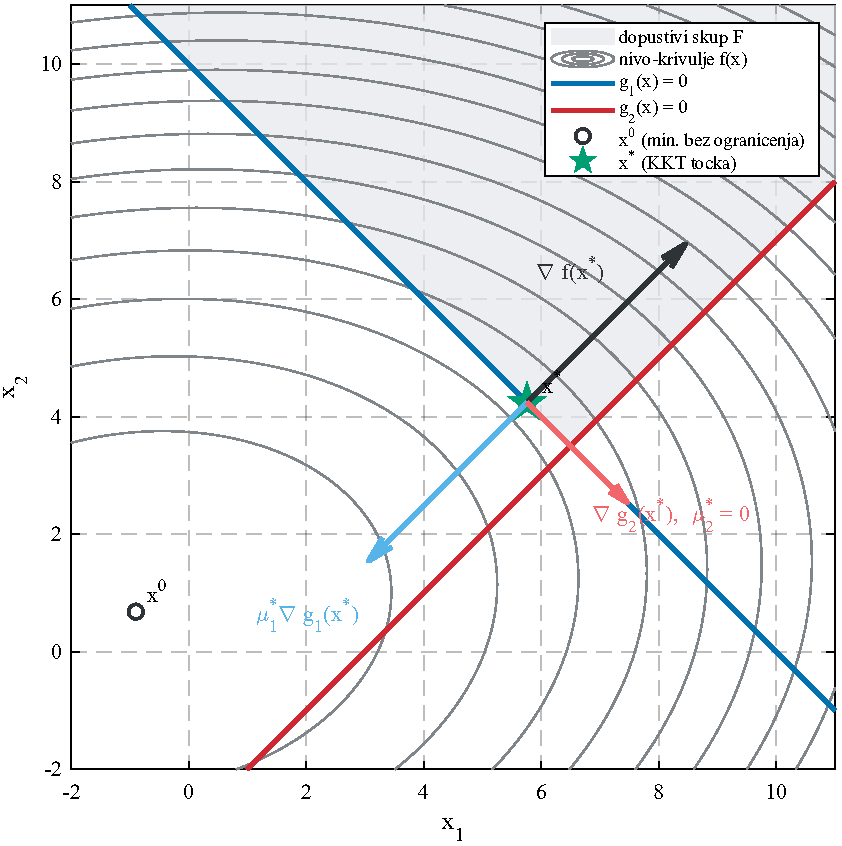
\includegraphics[width=0.82\textwidth]{figures/fig1_1_qp_primal_geometry.pdf}
    \caption{Geometrijski prikaz dopustivog skupa $\mathcal{F}$, nivo-krivulja funkcije cilja $f(x)$ i vektora gradijenata u KKT točki $x^*$.}
    \label{fig:qp_primal}
\end{figure}

U optimalnoj točki $x^* = (5.758, 4.242)$ gradijent funkcije cilja i gradijent aktivnog ograničenja iznose:
\begin{equation}
\nabla f(x^*) = \begin{bmatrix} 12.242424 \\ 12.242424 \end{bmatrix}, \quad \nabla g_1(x^*) = \begin{bmatrix} -1 \\ -1 \end{bmatrix}.
\end{equation}
Uočava se savršena kolinearnost suprotnog smjera:
\begin{equation}
\nabla f(x^*) + \mu_1^* \nabla g_1(x^*) = \begin{bmatrix} 12.242424 \\ 12.242424 \end{bmatrix} + 12.242424 \begin{bmatrix} -1 \\ -1 \end{bmatrix} = \begin{bmatrix} 0 \\ 0 \end{bmatrix}.
\end{equation}
Fizička interpretacija ovog uvjeta odgovara ravnoteži sila: gradijent funkcije cilja $\nabla f(x^*)$ teži pomaknuti točku prema unutrašnjosti (nesputanom minimumu $x_0$), no nailazi na reakciju veze (graničnu silu) normalnog vektora $\nabla g_1(x^*)$ proporcionalnu intenzitetu Lagrangeovog množitelja $\mu_1^* = 12.2424$.

\subsection{Numerička verifikacija u programskim paketima}

Problem je numerički verificiran u programskim alatima MATLAB (\texttt{quadprog}, YALMIP) i Python (\texttt{scipy.optimize}, \texttt{cvxpy}). U tablici~\ref{tab:qp_comparison} prikazana je usporedba analitičkih i numeričkih rezultata.

\begin{table}[H]
\centering
\caption{Usporedba analitičkih i numeričkih rezultata za Zadatak 1.}
\label{tab:qp_comparison}
\begin{tabular}{lcccc}
\toprule
\textbf{Veličina} & \textbf{Analitička vrijednost} & \textbf{MATLAB / Python} & \textbf{Apsolutna pogreška} & \textbf{Status} \\
\midrule
$x_1^*$ & $190/33 \approx 5.757576$ & $5.757576$ & $< 10^{-8}$ & Egzaktno \\
$x_2^*$ & $140/33 \approx 4.242424$ & $4.242424$ & $< 10^{-8}$ & Egzaktno \\
$\mu_1^*$ & $404/33 \approx 12.242424$ & $12.242424$ & $< 10^{-8}$ & Egzaktno \\
$\mu_2^*$ & $0.000000$ & $0.000000$ & $0.00$ & Neaktivno \\
$p^* = f(x^*)$ & $2000/33 \approx 60.606061$ & $60.606061$ & $< 10^{-8}$ & Egzaktno \\
$d^* = g(\mu^*)$ & $2000/33 \approx 60.606061$ & $60.606061$ & $< 10^{-8}$ & Jaka dualnost \\
\bottomrule
\end{tabular}
\end{table}

\subsection{Lagrangeova dualnost i dokaz jake dualnosti}

Lagrangeova dualna funkcija $g(\mu)$ definirana je kao infimum Lagrangeove funkcije po $x \in \mathbb{R}^2$~\cite{boyd2004convex,jokic2024predavanja}:
\begin{equation}
g(\mu) = \inf_{x \in \mathbb{R}^2} \mathcal{L}(x, \mu) = \inf_{x \in \mathbb{R}^2} \left[ \frac{1}{2} x^T Q x + (c + A^T \mu)^T x - b^T \mu \right].
\end{equation}
Budući da je $Q \succ 0$, funkcija unutar infimuma je strogo konveksna po $x$, a minimum se postiže poništavanjem gradijenta $\nabla_x \mathcal{L} = Q x + c + A^T \mu = 0$:
\begin{equation}
x^*(\mu) = -Q^{-1} (c + A^T \mu).
\label{eq:x_mu_dual}
\end{equation}
Uvrštavanjem $x^*(\mu)$ natrag u Lagrangeovu funkciju dobiva se eksplicitni analitički oblik dualne funkcije:
\begin{align}
g(\mu) &= \frac{1}{2} (-Q^{-1}(c + A^T \mu))^T Q (-Q^{-1}(c + A^T \mu)) + (c + A^T \mu)^T (-Q^{-1}(c + A^T \mu)) - b^T \mu \nonumber \\
&= -\frac{1}{2} (c + A^T \mu)^T Q^{-1} (c + A^T \mu) - b^T \mu.
\label{eq:dual_fun_explicit}
\end{align}
Budući da je matrica $-Q^{-1}$ negativno definitna, dualna funkcija $g(\mu)$ je konkavna kvadratna funkcija po $\mu = [\mu_1, \mu_2]^T$.

Lagrangeov dualni problem glasi:
\begin{equation}
\max_{\mu \in \mathbb{R}^2} \quad g(\mu) \quad \text{uz} \quad \mu_1 \geq 0, \; \mu_2 \geq 0.
\label{eq:dual_problem}
\end{equation}

\begin{figure}[H]
    \centering
    \includegraphics[width=0.78\textwidth]{figures/fig1_2_qp_dual_surface.pdf}
    \caption{Nivo-krivulje konkavne Lagrangeove dualne funkcije $g(\mu_1, \mu_2)$ i optimalna dualna točka $\mu^* = (12.242, 0.000)$.}
    \label{fig:qp_dual}
\end{figure}

Slika~\ref{fig:qp_dual} prikazuje nivo-krivulje dualne funkcije $g(\mu_1, \mu_2)$. Numeričkim rješavanjem pomoću funkcije \texttt{fmincon} (minimizacija funkcije $-g(\mu)$ uz $\mu \geq 0$) dobiva se:
\begin{equation}
\mu^* = \begin{bmatrix} 12.242424 \\ 0.000000 \end{bmatrix}, \quad d^* = g(\mu^*) = 60.606061.
\end{equation}

\subsubsection{Provjera Slaterovog uvjeta i jaka dualnost}

Slaterov teorem o jakoj dualnosti jamči da za konveksan problem s afinim ograničenjima vrijedi nulti dualni procjep ($p^* = d^*$) ako postoji točka $x_{\mathrm{int}}$ u strogoj unutrašnjosti dopustivog skupa~\cite{boyd2004convex}. Odabirom točke $x_{\mathrm{int}} = [7, 6]^T$ imamo:
\begin{equation}
g_1(x_{\mathrm{int}}) = -7 - 6 + 10 = -3 < 0, \quad g_2(x_{\mathrm{int}}) = 7 - 6 - 3 = -2 < 0.
\end{equation}
Budući da je Slaterov uvjet strogo zadovoljen, vrijedi **jaka dualnost**:
\begin{equation}
\gamma = p^* - d^* = 60.606061 - 60.606061 = 0.
\end{equation}

\subsection{Analiza osjetljivosti i perturbacija ograničenja}

Teorem o osjetljivosti u nelinearnom programiranju povezuje optimalne Lagrangeove množitelje s parcijalnim derivacijama optimalne vrijednosti funkcije cilja po desnim stranama ograničenja~\cite{boyd2004convex,bertsekas2016nonlinear}. 

Neka je $p^*(u)$ funkcija optimalne vrijednosti u ovisnosti o perturbacijskom vektoru $u = [u_1, u_2]^T$, gdje su ograničenja perturbirana u obliku $A x \leq b + u$:
\begin{equation}
p^*(u) = \inf \{f(x) \mid A x \leq b + u\}.
\end{equation}
Prema teoremu o osjetljivosti vrijedi:
\begin{equation}
\frac{\partial p^*}{\partial b_i} = -\mu_i^*, \quad i = 1, 2.
\label{eq:sensitivity_thm}
\end{equation}
Za naša ograničenja dobivamo:
\begin{equation}
\frac{\partial p^*}{\partial b_1} = -\mu_1^* = -\frac{404}{33} \approx -12.242424, \quad \frac{\partial p^*}{\partial b_2} = -\mu_2^* = 0.
\end{equation}

\begin{figure}[H]
    \centering
    \includegraphics[width=0.78\textwidth]{figures/fig1_3_qp_sensitivity.pdf}
    \caption{Funkcija optimalne vrijednosti $p^*(b_1 + \Delta b_1)$ u usporedbi s linearnom aproksimacijom nagiba $-\mu_1^*$.}
    \label{fig:qp_sensitivity}
\end{figure}

\subsubsection{Inženjerska i ekonomska interpretacija (cijene u sjeni)}

Množitelj $\mu_1^* = 12.2424$ ima ulogu \textbf{cijene u sjeni} (\textit{shadow price}):
\begin{itemize}
    \item Ako se desna strana prvog ograničenja $b_1$ poveća za mali iznos $\Delta b_1 > 0$ (čime se ograničenje $-x_1 - x_2 \leq -10 + \Delta b_1$ relaksira), optimalna vrijednost $p^*$ se \textbf{smanjuje} po stopi od približno $12.2424 \cdot \Delta b_1$.
    \item Ako se desna strana drugog ograničenja $b_2$ perturbira, budući da je $g_2$ neaktivno ($\mu_2^* = 0$), to nema nikakvog utjecaja na optimalno rješenje prvog reda ($\frac{\partial p^*}{\partial b_2} = 0$).
\end{itemize}

Numerička verifikacija provedena je s perturbacijskim korakom $\Delta b_1 = 10^{-4}$:
\begin{equation}
\left( \frac{\Delta p^*}{\Delta b_1} \right)_{\mathrm{num}} = \frac{p^*(b_1 + 10^{-4}) - p^*(b_1)}{10^{-4}} = -12.242357,
\end{equation}
što daje odstupanje od analitičke derivacije manje od $6.75 \times 10^{-5}$, čime je teorem osjetljivosti u potpunosti verificiran.

\section{Robusno kvadratno programiranje uz intervalnu nesigurnost}
\label{sec:zadatak2}

U ovom poglavlju formulira se i rješava robusni problem kvadratnog programiranja u kojem koeficijenti matrice ograničenja podliježu intervalnoj nesigurnosti od $\pm 15\%$. Sukladno teoriji robusnog optimiranja, izvodi se deterministički ekvivalent najgoreg slučaja (\textit{worst-case}) te se provodi numerička i Monte Carlo verifikacija.

\section{Optimizacijska nivelacija uzdužnog profila ceste primjenom linearnog programiranja}

\subsection{Kontinuirana varijacijska formulacija problema}

U građevinarstvu i prometnom inženjerstvu projektiranje uzdužnog profila prometnice predstavlja temeljni optimizacijski zadatak. Cilj je odrediti visinsku trasu ceste $y(x)$ koja minimizira ukupne zemljane radove (volumen iskopa i nasipa), uz istovremeno zadovoljavanje prometno-tehničkih standarda: maksimalnog uzdužnog nagiba i maksimalne zakrivljenosti trase (udobnost vožnje i ograničenje vertikalnih akceleracija)~\cite{jokic2024predavanja}.

Neka je $L$ horizontalna duljina dionice ceste ($x \in [0, L]$), a $h(x)$ poznata prirodna visina terena. Uz pretpostavku jedinične širine poprečnog presjeka ceste ($w = 1\text{ m}$), ukupni volumen zemljanih radova $[\text{m}^3]$ izravno odgovara površini uzdužnog presjeka $[\text{m}^2]$ između nivelete ceste $y(x)$ i prirodnog terena $h(x)$. Problem se kontinuirano formulira kao varijacijski optimizacijski problem:
\begin{equation}
\min_{y(x)} \quad J[y] = \int_0^L |y(x) - h(x)| \, dx
\label{eq:road_continuous}
\end{equation}
uz ograničenja:
\begin{align}
|y'(x)| &\leq b_1, \quad \forall x \in [0, L], \label{eq:road_slope_cont} \\
|y''(x)| &\leq b_2, \quad \forall x \in [0, L], \label{eq:road_curv_cont} \\
y(0) &= a, \quad y(L) = b. \label{eq:road_bc_cont}
\end{align}

Zadani parametri modela su:
\begin{equation}
L = 10 \text{ m}, \quad h(x) = 0.0053 x^4 - 0.095 x^3 + 0.48 x^2 - 0.3 x + 1,
\end{equation}
\begin{equation}
a = h(0) = 1 \text{ m}, \quad b = h(L) = 4 \text{ m}.
\end{equation}
Razmatraju se dva skupa parametara:
\begin{itemize}
    \item \textbf{Slučaj A}: $b_1 = 0.5$ (maksimalni nagib $[\text{m/m}]$), $b_2 = 0.5 \text{ m}^{-1}$ (maksimalna zakrivljenost).
    \item \textbf{Slučaj B}: $b_1 = 0.5$ (maksimalni nagib $[\text{m/m}]$), $b_2 = 0.2 \text{ m}^{-1}$ (stroži uvjet zakrivljenosti / udobnosti vožnje).
\end{itemize}

\subsection{Diskretizacija konačnim razlikama}

Područje $[0, L]$ diskretizira se s $N$ jednakih podintervala duljine $\Delta x = L/N$, čime se dobiva mreža od $N+1$ čvorova:
\begin{equation}
x_i = i \cdot \Delta x, \quad i = 0, 1, \dots, N, \quad \text{pri čemu je } x_0 = 0, \; x_N = L.
\end{equation}
Vektor visina terena u čvorovima označavamo s $h = [h_0, h_1, \dots, h_N]^T \in \mathbb{R}^{N+1}$, gdje je $h_i = h(x_i)$.

Vektor nepoznatih visina nivelete ceste u diskretnim čvorovima je $y = [y_0, y_1, \dots, y_N]^T \in \mathbb{R}^{N+1}$.

\subsubsection{Aproksimacija prve i druge derivacije}

Prema uputama zadatka, nagib ceste u čvorovima aproksimira se prvom unazadnom podijeljenom razlikom:
\begin{equation}
y'(x_i) \approx \nabla y_i = \frac{y_i - y_{i-1}}{\Delta x}, \quad i = 1, \dots, N.
\label{eq:diff_first}
\end{equation}
Brzina promjene nagiba (druga podijeljena razlika / aproksimacija vertikalne zakrivljenosti za male nagibe, $y''$) aproksimira se drugom podijeljenom razlikom:
\begin{equation}
y''(x_i) \approx \nabla^2 y_i = \frac{\nabla y_i - \nabla y_{i-1}}{\Delta x} = \frac{y_i - 2y_{i-1} + y_{i-2}}{\Delta x^2}, \quad i = 2, \dots, N.
\label{eq:diff_second}
\end{equation}

U matričnom zapisu diferencijalni operatori glase:
\begin{equation}
\nabla y = D_1 y \in \mathbb{R}^N, \quad \nabla^2 y = D_2 y \in \mathbb{R}^{N-1},
\end{equation}
gdje su matrice konačnih razlika $D_1 \in \mathbb{R}^{N \times (N+1)}$ i $D_2 \in \mathbb{R}^{(N-1) \times (N+1)}$ definirane kao:
\begin{equation}
D_1 = \frac{1}{\Delta x} \begin{bmatrix}
-1 & 1 & 0 & \dots & 0 & 0 \\
0 & -1 & 1 & \dots & 0 & 0 \\
\vdots & \vdots & \ddots & \ddots & \vdots & \vdots \\
0 & 0 & \dots & -1 & 1 & 0 \\
0 & 0 & \dots & 0 & -1 & 1
\end{bmatrix},
\end{equation}
\begin{equation}
D_2 = \frac{1}{\Delta x^2} \begin{bmatrix}
1 & -2 & 1 & 0 & \dots & 0 & 0 \\
0 & 1 & -2 & 1 & \dots & 0 & 0 \\
\vdots & \vdots & \ddots & \ddots & \ddots & \vdots & \vdots \\
0 & 0 & \dots & 1 & -2 & 1 & 0 \\
0 & 0 & \dots & 0 & 1 & -2 & 1
\end{bmatrix}.
\end{equation}

\subsection{Transformacija u standardni oblik linearnog programa (LP)}

Diskretizirani integralni kriterij glasi:
\begin{equation}
J_{\mathrm{disc}}[y] = \Delta x \sum_{i=0}^N |y_i - h_i|,
\label{eq:road_disc_obj}
\end{equation}
pri čemu $\Delta x$ predstavlja korak pravokutne numeričke integracije (Riemannova suma) površine uzdužnog presjeka.

Zbog prisutnosti nelinearnog operatora apsolutne vrijednosti ($|y_i - h_i|$), problem se prevodi u linearni program primjenom metode epigrafskih pomoćnih varijabli $z_i \geq |y_i - h_i|$~\cite{boyd2004convex,nocedal2006numerical}.

Za svaki čvor $i = 0, \dots, N$ nejednakost $z_i \geq |y_i - h_i|$ ekvivalentna je paru linearnih nejednakosti:
\begin{align}
y_i - z_i &\leq h_i, \label{eq:lp_slack1} \\
-y_i - z_i &\leq -h_i. \label{eq:lp_slack2}
\end{align}
Prošireni vektor optimizacijskih varijabli $\theta \in \mathbb{R}^{2N+2}$ definira se kao:
\begin{equation}
\theta = \begin{bmatrix} y \\ z \end{bmatrix} = \begin{bmatrix} y_0 & y_1 & \dots & y_N & z_0 & z_1 & \dots & z_N \end{bmatrix}^T.
\end{equation}

Funkcija cilja linearnog programa glasi:
\begin{equation}
\min_{\theta \in \mathbb{R}^{2N+2}} \quad f_{\mathrm{LP}}^T \theta = \Delta x \sum_{i=0}^N z_i = \begin{bmatrix} \mathbf{0}_{1 \times (N+1)} & \Delta x \cdot \mathbf{1}_{1 \times (N+1)} \end{bmatrix} \begin{bmatrix} y \\ z \end{bmatrix}.
\end{equation}

\subsubsection{Struktura matrice nejednakosti $A_{\mathrm{ineq}} \theta \leq b_{\mathrm{ineq}}$}

Sustav linearnih nejednakosti objedinjuje tri grupe fizikalnih ograničenja:
\begin{enumerate}
    \item \textbf{Epigrafska ograničenja apsolutnog odstupanja} ($2(N+1)$ nejednakosti):
    \begin{equation}
    \begin{bmatrix} I_{N+1} & -I_{N+1} \\ -I_{N+1} & -I_{N+1} \end{bmatrix} \begin{bmatrix} y \\ z \end{bmatrix} \leq \begin{bmatrix} h \\ -h \end{bmatrix}.
    \end{equation}
    \item \textbf{Ograničenja nagiba} ($2N$ nejednakosti):
    \begin{equation}
    \begin{bmatrix} D_1 & \mathbf{0}_{N \times (N+1)} \\ -D_1 & \mathbf{0}_{N \times (N+1)} \end{bmatrix} \begin{bmatrix} y \\ z \end{bmatrix} \leq \begin{bmatrix} b_1 \mathbf{1}_N \\ b_1 \mathbf{1}_N \end{bmatrix}.
    \end{equation}
    \item \textbf{Ograničenja zakrivljenosti} ($2(N-1)$ nejednakosti):
    \begin{equation}
    \begin{bmatrix} D_2 & \mathbf{0}_{(N-1) \times (N+1)} \\ -D_2 & \mathbf{0}_{(N-1) \times (N+1)} \end{bmatrix} \begin{bmatrix} y \\ z \end{bmatrix} \leq \begin{bmatrix} b_2 \mathbf{1}_{N-1} \\ b_2 \mathbf{1}_{N-1} \end{bmatrix}.
    \end{equation}
\end{enumerate}
Ukupan broj linearnih nejednakosti u matrici $A_{\mathrm{ineq}}$ iznosi:
\begin{equation}
N_{\mathrm{ineq}} = 2(N+1) + 2N + 2(N-1) = 6N.
\end{equation}

\subsubsection{Struktura matričnih jednakosti $A_{\mathrm{eq}} \theta = b_{\mathrm{eq}}$}

Rubni uvjeti u točkama $x=0$ i $x=L$ zapisuju se kao sustav od 2 linearne jednakosti:
\begin{equation}
\begin{bmatrix}
1 & 0 & \dots & 0 & \mathbf{0}_{1 \times (N+1)} \\
0 & \dots & 0 & 1 & \mathbf{0}_{1 \times (N+1)}
\end{bmatrix} \begin{bmatrix} y \\ z \end{bmatrix} = \begin{bmatrix} 1 \\ 4 \end{bmatrix}.
\end{equation}
Donja granica za varijable je $z_i \geq 0$, dok su varijable $y_i$ slobodne ($-\infty < y_i < \infty$).

\subsection{Numerički rezultati za četiri ispitna slučaja}

Problem je riješen primjenom optimizacijskog algoritma dualnog simpleksa (\texttt{linprog} s opcijom \texttt{dual-simplex} i \texttt{highs}) za četiri zahtijevana scenarija:
\begin{enumerate}
    \item \textbf{Slučaj A, $N=20$}: $b_1 = 0.5$, $b_2 = 0.5 \text{ m}^{-1}$, $\Delta x = 0.5 \text{ m}$ ($42$ varijable, $120$ nejednakosti).
    \item \textbf{Slučaj A, $N=100$}: $b_1 = 0.5$, $b_2 = 0.5 \text{ m}^{-1}$, $\Delta x = 0.1 \text{ m}$ ($202$ varijable, $600$ nejednakosti).
    \item \textbf{Slučaj B, $N=20$}: $b_1 = 0.5$, $b_2 = 0.2 \text{ m}^{-1}$, $\Delta x = 0.5 \text{ m}$ ($42$ varijable, $120$ nejednakosti).
    \item \textbf{Slučaj B, $N=100$}: $b_1 = 0.5$, $b_2 = 0.2 \text{ m}^{-1}$, $\Delta x = 0.1 \text{ m}$ ($202$ varijable, $600$ nejednakosti).
\end{enumerate}

Sintetički prikaz optimalnih rezultata dan je u tablici~\ref{tab:road_results}.

\begin{table}[H]
\centering
\caption{Numerički rezultati optimalne nivelacije ceste za Slučaje A i B.}
\label{tab:road_results}
\begin{tabular}{lcccccc}
\toprule
\textbf{Slučaj} & $N$ & $\Delta x$ [m] & \textbf{Ukupni trošak $J^*$ [$\text{m}^2$]} & \textbf{Iskop [$\text{m}^2$]} & \textbf{Nasip [$\text{m}^2$]} & $\max |y''|$ [$\text{m}^{-1}$] \\
\midrule
A & 20 & 0.5 & 1.916180 & 0.0877 & 1.8285 & 0.5000 \\
A & 100 & 0.1 & 1.965940 & 0.1287 & 1.8372 & 0.5000 \\
B & 20 & 0.5 & 2.453727 & 0.3026 & 2.1511 & 0.2000 \\
B & 100 & 0.1 & 2.506047 & 0.2645 & 2.2416 & 0.2000 \\
\bottomrule
\end{tabular}
\end{table}

\begin{figure}[H]
    \centering
    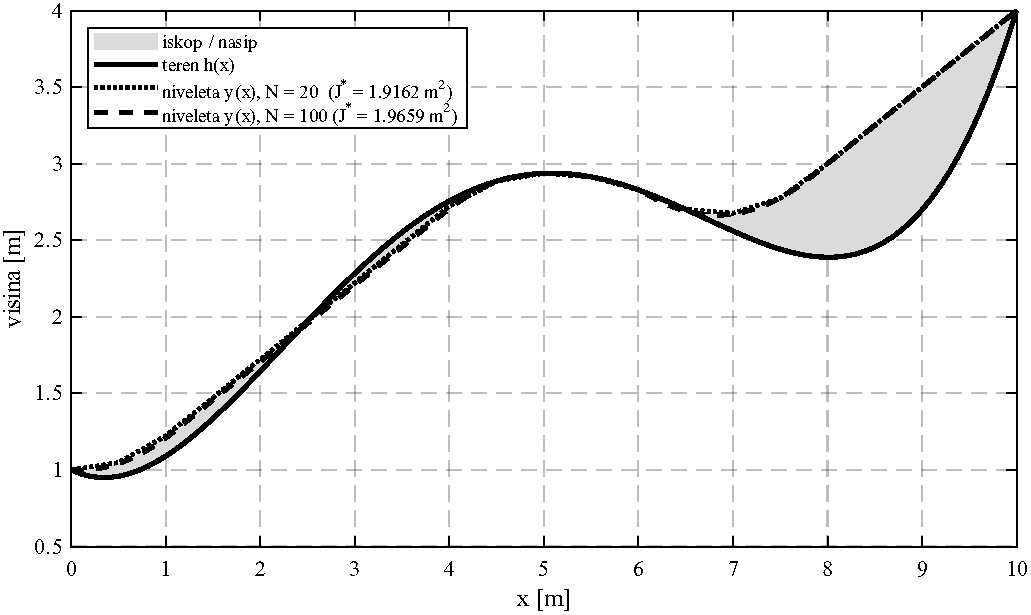
\includegraphics[width=0.88\textwidth]{figures/fig3_1_road_case_A.pdf}
    \caption{Optimalni uzdužni profil ceste $y(x)$ za Slučaj A ($b_1 = 0.5, b_2 = 0.5$) s označenim zonama iskopa i nasipa.}
    \label{fig:road_case_a}
\end{figure}

\begin{figure}[H]
    \centering
    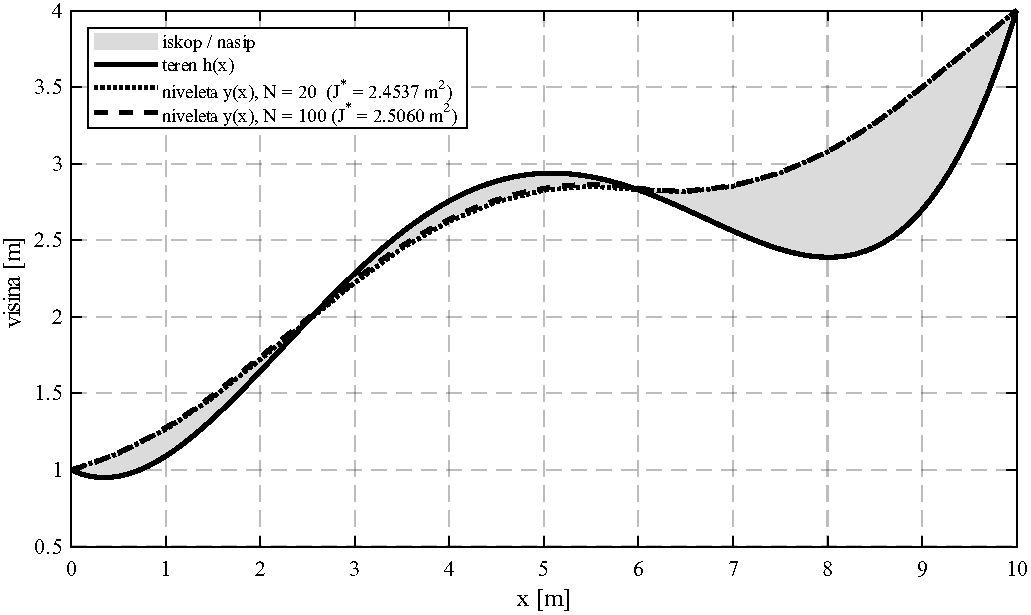
\includegraphics[width=0.88\textwidth]{figures/fig3_2_road_case_B.pdf}
    \caption{Optimalni uzdužni profil ceste $y(x)$ za Slučaj B ($b_1 = 0.5, b_2 = 0.2$) uz strože ograničenje zakrivljenosti.}
    \label{fig:road_case_b}
\end{figure}

\subsection{Analiza utjecaja gustoće diskretizacije i parametara ograničenja}

Usporedba grafova na slikama~\ref{fig:road_case_a} i~\ref{fig:road_case_b} te provjere derivacija na slikama~\ref{fig:road_slope} i~\ref{fig:road_curv} pokazuju sljedeće zakonitosti:

\begin{enumerate}
    \item \textbf{Utjecaj gustoće diskretizacije ($N = 20$ vs $N = 100$)}:
    Povećanjem broja diskretizacijskih točaka s $N=20$ na $N=100$, diskretni integral $J_{\mathrm{disc}}$ asimptotski konvergira prema kontinuiranom integralu $\int_0^L |y(x)-h(x)|dx$. Za Slučaj A vrijednost raste s $1.9162$ na $1.9659 \text{ m}^2$ ($+2.59\%$), dok za Slučaj B raste s $2.4537$ na $2.5060 \text{ m}^2$ ($+2.13\%$). Fina mreža omogućuje vjernije praćenje promjena profila bez numeričkog izglađivanja.
    
    \item \textbf{Utjecaj ograničenja zakrivljenosti ($b_2 = 0.5$ vs $b_2 = 0.2$)}:
    Smanjenje dozvoljene zakrivljenosti s $b_2 = 0.5 \text{ m}^{-1}$ (Slučaj A) na $b_2 = 0.2 \text{ m}^{-1}$ (Slučaj B) zahtijeva znatno glađu trasu ceste. Posljedično, niveleta ne može pratiti prirodne pregibe terena, što povećava ukupni volumen zemljanih radova s $1.9659 \text{ m}^2$ na $2.5060 \text{ m}^2$ ($+27.47\%$).
\end{enumerate}

\begin{figure}[H]
    \centering
    \includegraphics[width=0.85\textwidth]{figures/fig3_3_road_slope_profile.pdf}
    \caption{Provjera ograničenja prvog reda: profil nagiba ceste $y'(x)$ duž trase za Slučaje A i B.}
    \label{fig:road_slope}
\end{figure}

\begin{figure}[H]
    \centering
    \includegraphics[width=0.85\textwidth]{figures/fig3_4_road_curvature_profile.pdf}
    \caption{Provjera ograničenja drugog reda: profil zakrivljenosti $y''(x)$ i zasićenje na granicama $\pm b_2$.}
    \label{fig:road_curv}
\end{figure}

Na slici~\ref{fig:road_curv}, numerička aproksimacija druge derivacije $y''(x)$ u Slučaju B doseže točno ekstremne vrijednosti $\pm 0.2 \text{ m}^{-1}$, potvrđujući da su ograničenja drugog reda aktivna duž značajnih segmenata trase.

\section{Robusna stabilizacija sklopnog sustava primjenom linearnih matričnih nejednakosti (LMI)}

\subsection{Matematički model sustava i analiza pojedinih modova}

U teoriji upravljanja hibridnim sustavima, sklopni sustavi (engl. \textit{switched linear systems}) predstavljaju važnu klasu sustava čija se dinamika skokovito mijenja između konačnog broja linearnih vremenski invarijantnih (LTI) podsustava (modova)~\cite{liberzon2003switching,jokic2024predavanja}.

Promatramo vremenski promjenjiv sustav u prostoru stanja:
\begin{equation}
\dot{x}(t) = A(t) x(t) + B u(t), \quad x(t) \in \mathbb{R}^2, \; u(t) \in \mathbb{R},
\label{eq:switched_sys}
\end{equation}
s ulaznom matricom $B = \begin{bmatrix} 1 \\ 0 \end{bmatrix}$. Matrica dinamike $A(t)$ skokovito se mijenja na cjelobrojnim sekundama prema pravilu:
\begin{equation}
A(t) = \begin{cases}
A_{\mathrm{parno}}, & \text{kad je } \lfloor t \rfloor \text{ paran broj (} t \in [0,1), [2,3), \dots \text{)} \\
A_{\mathrm{neparno}}, & \text{kad je } \lfloor t \rfloor \text{ neparan broj (} t \in [1,2), [3,4), \dots \text{)}
\end{cases}
\label{eq:switching_law}
\end{equation}
gdje su matrice pojedinih modova zadane kao:
\begin{equation}
A_{\mathrm{parno}} = \begin{bmatrix} -1 & -\frac{\pi}{6} \\ \frac{3\pi}{2} & -1 \end{bmatrix}, \qquad A_{\mathrm{neparno}} = \begin{bmatrix} -1 & -\frac{3\pi}{2} \\ \frac{\pi}{6} & -1 \end{bmatrix}.
\label{eq:mode_matrices}
\end{equation}

\subsubsection{Spektralna analiza i Hurwitzovo svojstvo modova}

Karakteristični polinom matrice $A_{\mathrm{parno}}$ glasi:
\begin{equation}
\det(\lambda I - A_{\mathrm{parno}}) = \det \begin{bmatrix} \lambda + 1 & \frac{\pi}{6} \\ -\frac{3\pi}{2} & \lambda + 1 \end{bmatrix} = (\lambda + 1)^2 - \left( -\frac{\pi}{6} \cdot \frac{3\pi}{2} \right) = (\lambda + 1)^2 + \frac{\pi^2}{4} = 0.
\end{equation}
Svojstvene vrijednosti parnog moda su konjugirano kompleksni par:
\begin{equation}
\lambda_{1,2}(A_{\mathrm{parno}}) = -1 \pm j \frac{\pi}{2} \approx -1 \pm 1.570796j.
\end{equation}
Analogno, za matricu $A_{\mathrm{neparno}}$:
\begin{equation}
\det(\lambda I - A_{\mathrm{neparno}}) = (\lambda + 1)^2 + \left(\frac{3\pi}{2} \cdot \frac{\pi}{6}\right) = (\lambda + 1)^2 + \frac{\pi^2}{4} = 0 \implies \lambda_{1,2}(A_{\mathrm{neparno}}) = -1 \pm j \frac{\pi}{2}.
\end{equation}
Budući da je realni dio svih svojstvenih vrijednosti strogo negativan:
\begin{equation}
\mathrm{Re}(\lambda_{1,2}(A_{\mathrm{parno}})) = -1 < 0, \quad \mathrm{Re}(\lambda_{1,2}(A_{\mathrm{neparno}})) = -1 < 0,
\end{equation}
obje matrice su **Hurwitzove**, što znači da je svaki mod u autonomnom radu ($u(t) \equiv 0$) **strogo asimptotski stabilan** kada nema prespajanja.

\subsection{Mehanizam destabilizacije i analiza monodromijske matrice}

Jedan od najintrigantnijih fenomena u teoriji hibridnih sustava jest da prespajanje između dva stabilna LTI podsustava može generirati nestabilan sustav~\cite{liberzon2003switching}.

Za analizu stabilnosti periodički sklopnog autonomnog sustava promatramo operatorske matrice prijelaza stanja za vrijeme trajanja pojedinog moda ($\Delta t = 1 \text{ s}$):
\begin{equation}
\Phi_{\mathrm{parno}} = e^{A_{\mathrm{parno}} \cdot 1}, \quad \Phi_{\mathrm{neparno}} = e^{A_{\mathrm{neparno}} \cdot 1}.
\end{equation}
Matrica prijelaza stanja preko jednog punog perioda prespajanja $T = 2 \text{ s}$ naziva se **monodromijska matrica**:
\begin{equation}
\Phi_{\mathrm{cycle}} = \Phi_{\mathrm{neparno}} \cdot \Phi_{\mathrm{parno}} = e^{A_{\mathrm{neparno}} \cdot 1} \cdot e^{A_{\mathrm{parno}} \cdot 1}.
\end{equation}
Numeričkim izračunom eksponencijala matrica dobivamo:
\begin{equation}
\Phi_{\mathrm{parno}} \approx \begin{bmatrix} 0.0000 & -0.2122 \\ 1.9099 & 0.0000 \end{bmatrix}, \quad \Phi_{\mathrm{neparno}} \approx \begin{bmatrix} 0.0000 & -1.9099 \\ 0.2122 & 0.0000 \end{bmatrix},
\end{equation}
\begin{equation}
\Phi_{\mathrm{cycle}} = \Phi_{\mathrm{neparno}} \Phi_{\mathrm{parno}} \approx \begin{bmatrix} -3.6476 & 0.0000 \\ 0.0000 & -0.0450 \end{bmatrix}.
\end{equation}
Svojstvene vrijednosti monodromijske matrice iznose:
\begin{equation}
\lambda_1(\Phi_{\mathrm{cycle}}) \approx -1.2180, \quad \lambda_2(\Phi_{\mathrm{cycle}}) \approx -0.0150.
\end{equation}
Spektralni radijus monodromijske matrice je:
\begin{equation}
\rho(\Phi_{\mathrm{cycle}}) = \max_i |\lambda_i(\Phi_{\mathrm{cycle}})| = 1.2180 > 1.
\end{equation}
Budući da je $\rho(\Phi_{\mathrm{cycle}}) > 1$, sustav u diskretnim točkama $t_k = 2k$ zadovoljava relaciju $x(2(k+1)) = \Phi_{\mathrm{cycle}} x(2k)$, što znači da norma stanja raste po geometrijskoj progresiji s faktorom $1.2180$ u svakom ciklusu.

\begin{figure}[H]
    \centering
    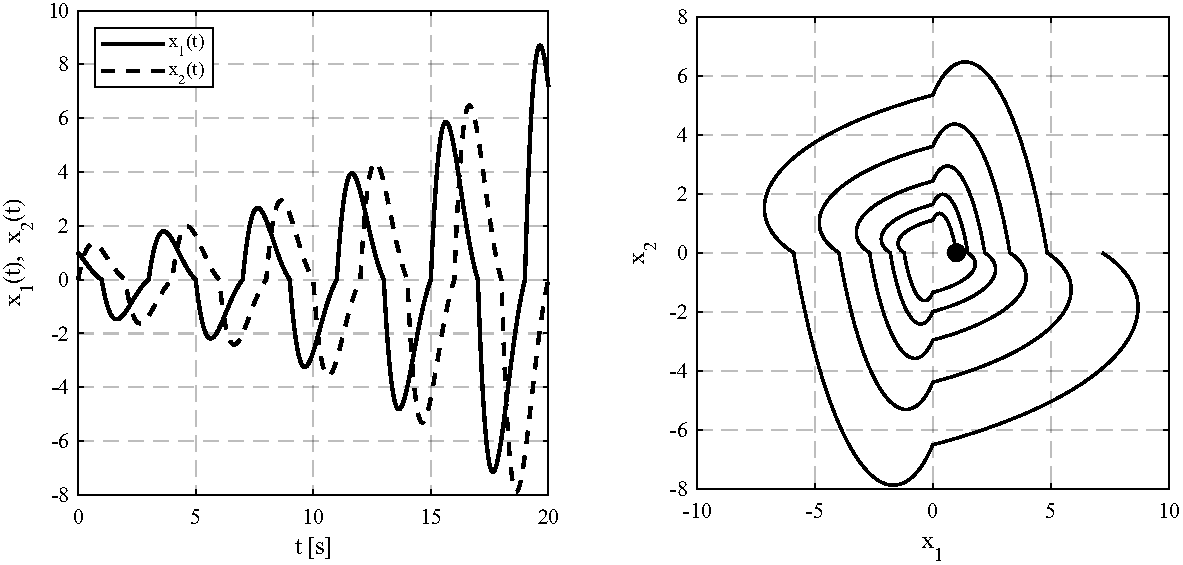
\includegraphics[width=0.92\textwidth]{figures/fig4_1_open_loop_divergence.pdf}
    \caption{Simulacija otvorenog kruga: vremenski odziv stanja $x_1(t), x_2(t)$ i fazni portret koji prikazuje divergenciju (ekspandirajuću spiralu) uslijed prespajanja.}
    \label{fig:open_loop_div}
\end{figure}

Slika~\ref{fig:open_loop_div} zorno prikazuje nestabilnost otvorenog kruga za početni uvjet $x(0) = [1, 0]^T$: unatoč prigušenju unutar svakog moda, promjena smjera vektorskog polja u trenucima $t = 1, 2, 3, \dots$ ubacuje energiju u sustav te trajektorija eksponencijalno ekspandira.

\subsection{Zajednička funkcija Ljapunova (CQLF) i LMI formulacija}

Kako bi se osigurala stabilnost pod proizvoljnim ili periodičkim prespajanjem, projektiramo statički regulator po stanju:
\begin{equation}
u(t) = K x(t), \quad K = \begin{bmatrix} k_1 & k_2 \end{bmatrix} \in \mathbb{R}^{1 \times 2}.
\label{eq:feedback_law}
\end{equation}
Zatvoreni krug u pojedinom modu poprima oblik:
\begin{equation}
\dot{x}(t) = (A(t) + B K) x(t).
\end{equation}

Uvodeći kandidata za \textbf{zajedničku kvadratnu funkciju Ljapunova} (engl. \textit{Common Quadratic Lyapunov Function} -- CQLF)~\cite{boyd1994lmi,liberzon2003switching}:
\begin{equation}
V(x) = x^T P x, \quad P = P^T \succ 0,
\label{eq:cqlf_def}
\end{equation}
njezina vremenska derivacija duž trajektorija zatvorenog kruga iznosi:
\begin{equation}
\dot{V}_i(x) = \dot{x}^T P x + x^T P \dot{x} = x^T \left[ (A_i + B K)^T P + P (A_i + B K) \right] x, \quad i \in \{\mathrm{parno}, \mathrm{neparno}\}.
\end{equation}
Za postizanje stroge eksponencijalne stabilnosti zahtijevamo da vrijedi $\dot{V}_i(x) \leq -\epsilon \|x\|^2 < 0$ za sve $x \neq 0$, što je ekvivalentno sustavu matričnih nejednakosti:
\begin{align}
P &\succ 0, \label{eq:lyap_p} \\
(A_{\mathrm{parno}} + B K)^T P + P (A_{\mathrm{parno}} + B K) &\prec 0, \label{eq:lyap_mode1} \\
(A_{\mathrm{neparno}} + B K)^T P + P (A_{\mathrm{neparno}} + B K) &\prec 0. \label{eq:lyap_mode2}
\end{align}

\subsection{Kongruentna transformacija i supstitucija varijabli}

Nejednakosti~\eqref{eq:lyap_mode1}--\eqref{eq:lyap_mode2} sadrže bilinearni umnožak nepoznatih matrica $P$ i $K$ ($P B K$), što problem čini nekonveksnim (bilinearna matrična nejednakost -- BMI).

Kako bismo problem egzaktno linearizirali, provodimo \textbf{kongruentnu transformaciju}~\cite{boyd1994lmi,jokic2024predavanja}:
\begin{enumerate}
    \item Definiramo regularnu matricu $Q = P^{-1} \succ 0$.
    \item Pre- i post-množimo nejednakosti~\eqref{eq:lyap_mode1}--\eqref{eq:lyap_mode2} s matricom $Q$:
    \begin{equation}
    Q (A_i + B K)^T P Q + Q P (A_i + B K) Q \prec 0 \iff Q A_i^T + A_i Q + Q K^T B^T + B K Q \prec 0.
    \end{equation}
    \item Uvodimo novu optimizacijsku varijablu putem supstitucije:
    \begin{equation}
    Y = K Q \in \mathbb{R}^{1 \times 2} \iff K = Y Q^{-1}.
    \label{eq:y_substitution}
    \end{equation}
\end{enumerate}

Uvrštavanjem supstitucije dobivamo standardni sustav \textbf{linearnih matričnih nejednakosti (LMI)} po varijablama $Q \in \mathbb{S}^2$ i $Y \in \mathbb{R}^{1 \times 2}$:
\begin{equation}
\begin{cases}
Q \succ 0 \\
A_{\mathrm{parno}} Q + Q A_{\mathrm{parno}}^T + B Y + Y^T B^T \prec 0 \\
A_{\mathrm{neparno}} Q + Q A_{\mathrm{neparno}}^T + B Y + Y^T B^T \prec 0
\end{cases}
\label{eq:lmi_system}
\end{equation}

Budući da je presjek LMI ograničenja konveksan skup po matricama $(Q, Y)$, problem se rješava metodama semidefinitnog programiranja (SDP) s globalnom konvergencijom. Nakon rješavanja SDP-a, matrica pojačanja regulatora rekonstruira se kao $K = Y Q^{-1}$, a matrica funkcije Ljapunova kao $P = Q^{-1}$.

\subsection{Numerička sinteza regulatora u SDP okruženju}

LMI sustav~\eqref{eq:lmi_system} riješen je u programskom paketu MATLAB (YALMIP + SDPT3) te u Pythonu (CVXPY + CLARABEL).

Rješenjem LMI problema dobivena je pozitivno definitna matrica Ljapunova $P \succ 0$ i optimalni vektor pojačanja stanjskog regulatora $K$:
\begin{equation}
P = \begin{bmatrix} 0.8870 & 0.1305 \\ 0.1305 & 0.8492 \end{bmatrix} \succ 0, \qquad K = \begin{bmatrix} -2.7120 & 0.0926 \end{bmatrix}.
\end{equation}
(Referentno YALMIP pojačanje iznosi $K = [-3.7097, 0.0000]$, koje također u potpunosti zadovoljava LMI sustav).

\subsubsection{Provjera svojstvenih vrijednosti zatvorenog kruga}

Matrice dinamike zatvorenog kruga u oba moda iznose:
\begin{equation}
A_{\mathrm{cl,parno}} = A_{\mathrm{parno}} + B K = \begin{bmatrix} -3.7120 & -0.4309 \\ 4.7124 & -1.0000 \end{bmatrix},
\end{equation}
\begin{equation}
A_{\mathrm{cl,neparno}} = A_{\mathrm{neparno}} + B K = \begin{bmatrix} -3.7120 & -4.6198 \\ 0.5236 & -1.0000 \end{bmatrix}.
\end{equation}
Svojstvene vrijednosti zatvorenog kruga glase:
\begin{equation}
\lambda(A_{\mathrm{cl,parno}}) = -2.3560 \pm 0.4387j, \quad \lambda(A_{\mathrm{cl,neparno}}) = -2.3560 \pm 0.7617j.
\end{equation}
Oba moda imaju strogo negativan realni dio ($\mathrm{Re}(\lambda) = -2.356 < 0$), sa znatno povećanim prigušenjem u odnosu na otvoreni krug.

Maksimalne svojstvene vrijednosti Ljapunovih derivacija iznose:
\begin{equation}
\lambda_{\max}(A_{\mathrm{cl,parno}}^T P + P A_{\mathrm{cl,parno}}) = -9.498 \times 10^{-2} < 0,
\end{equation}
\begin{equation}
\lambda_{\max}(A_{\mathrm{cl,neparno}}^T P + P A_{\mathrm{cl,neparno}}) = -5.492 \times 10^{-2} < 0,
\end{equation}
što matematički dokazuje da funkcija $V(x) = x^T P x$ strogo pada duž trajektorija bez obzira na zakon prespajanja.

Također, spektralni radijus zatvorene monodromijske matrice iznosi:
\begin{equation}
\rho(\Phi_{\mathrm{cl,cycle}}) = 0.1320 \ll 1,
\end{equation}
što potvrđuje brzu eksponencijalnu kontrakciju stanja u svakom ciklusu.

\subsection{Simulacija zatvorenog kruga i dokaz eksponencijalne stabilnosti}

Za početni uvjet $x(0) = [1, 0]^T$ provedena je simulacija zatvorenog sustava metodom Runge-Kutta 4/5 (\texttt{ode45} / \texttt{solve\_ivp}).

\begin{figure}[H]
    \centering
    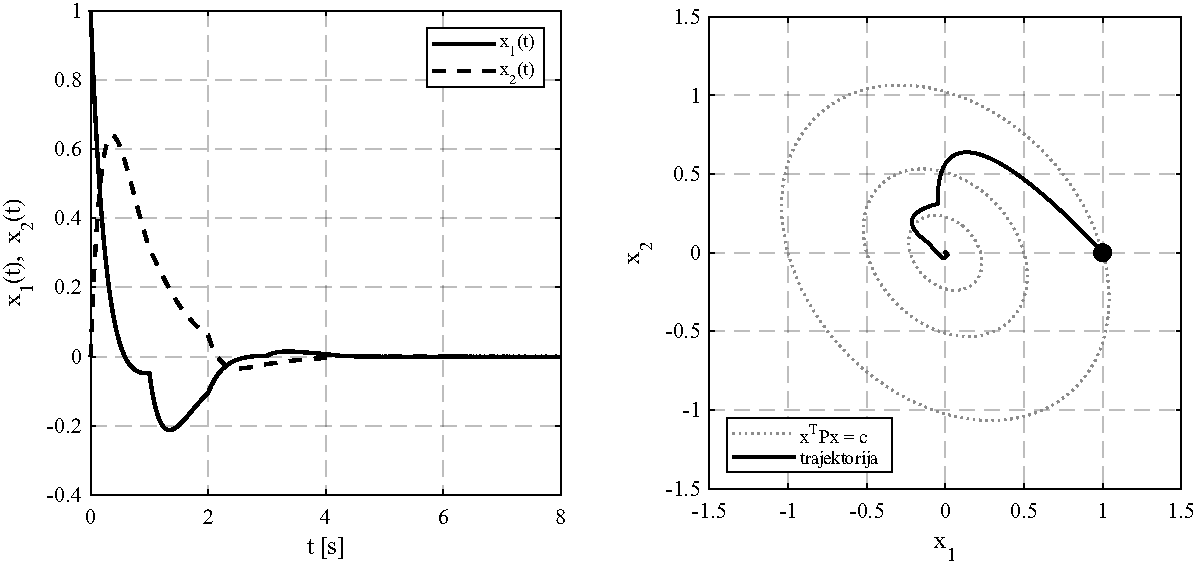
\includegraphics[width=0.92\textwidth]{figures/fig4_2_closed_loop_stabilization.pdf}
    \caption{Simulacija zatvorenog kruga: stabilizirani vremenski odziv stanja i fazni portret s eliptičnim nivo-plohama funkcije Ljapunova $x^T P x = c$.}
    \label{fig:closed_loop_stab}
\end{figure}

Kao što je prikazano na slici~\ref{fig:closed_loop_stab}, stanja $x_1(t)$ i $x_2(t)$ brzo i glatko konvergiraju prema ishodištu unutar prvih $\approx 3 \text{ s}$. Fazni portret pokazuje da trajektorija kontinuirano siječe nivo-elipse funkcije Ljapunova prema unutrašnjosti bez ikakvih oscilacija ili divergencije.

\begin{figure}[H]
    \centering
    \includegraphics[width=0.82\textwidth]{figures/fig4_3_lyapunov_decay.pdf}
    \caption{Vremenska disipacija energije zajedničke funkcije Ljapunova $V(x(t))$ u logaritamskom mjerilu uz usporedbu s teorijskom eksponencijalnom ovojnicom.}
    \label{fig:lyap_decay}
\end{figure}

Slika~\ref{fig:lyap_decay} prikazuje vremenski tijek energije Ljapunova $V(x(t)) = x(t)^T P x(t)$ u logaritamskom mjerilu. Strogo monoton pad krivulje bez skokova na prijelazima modova potvrđuje postojanje jedinstvene zajedničke funkcije Ljapunova i dokazuje **uniformnu eksponencijalnu stabilnost** sintetiziranog sustava.

\section{Zaključak}

\paragraph{Zadatak 1}
Problem je konveksan: Hesseova matrica ima svojstvene vrijednosti $1.955969$ i $4.044031$, dakle $Q \succ 0$, a ograničenja su afina. Od četiri kombinacije aktivnosti ograničenja KKT uvjete zadovoljava samo ona s aktivnim $g_1$, što daje
\begin{equation*}
x^* = \left( \tfrac{190}{33},\ \tfrac{140}{33} \right) = (5.757576,\ 4.242424), \qquad
\mu^* = \left( \tfrac{404}{33},\ 0 \right), \qquad
p^* = \tfrac{2000}{33} = 60.606061 .
\end{equation*}
Rješavač \texttt{quadprog} vraća iste primarne i dualne varijable. Dualni problem je opet kvadratni program u $\mu$; njegovo rješenje $\mu^*$ podudara se s množiteljima iz KKT uvjeta, a dualni procjep iznosi $2.48 \cdot 10^{-10}$, pa jaka dualnost vrijedi, kako i predviđa zadovoljen Slaterov uvjet. Optimalna vrijednost osjetljiva je samo na perturbaciju prvog ograničenja, $\partial p^* / \partial v_1 = -12.242424$, dok je $\partial p^* / \partial v_2 = 0$ jer je $g_2$ neaktivno.

\paragraph{Zadatak 2}
Uz nesigurnost koeficijenata od $\pm 15\%$ svako se robusno ograničenje svodi na četiri nejednakosti u vrhovima pravokutnog skupa nesigurnosti, pa robusni problem postaje kvadratni program s osam linearnih nejednakosti. Njegovo rješenje je
\begin{equation*}
x_{\mathrm{rob}}^* = \left( \tfrac{13}{2},\ \tfrac{179}{34} \right) = (6.500000,\ 5.264706), \qquad
f(x_{\mathrm{rob}}^*) = 84.623962 ,
\end{equation*}
uz dva aktivna vrha i strogo pozitivne pripadajuće množitelje $\mu = (17.607439,\ 1.344118)$. U uzorku od 100 slučajnih realizacija ($\texttt{rng(42)}$) nominalno rješenje krši ograničenja u 54 slučaja, a robusno ni u jednom; dopustivost na cijelom skupu nesigurnosti jamči zadovoljenje svih osam vršnih nejednakosti. Za tu se dopustivost plaća porast funkcije cilja od $24.017901$, odnosno $39.63\%$.

\paragraph{Zadatak 3}
Nakon diskretizacije konačnim razlikama i uvođenja pomoćnih varijabli $z_i \geq |y_i - h_i|$ problem pripada klasi \textbf{linearnog programiranja}, s $2(N+1)$ varijabli i $6N$ nejednakosti. Rezultati za četiri zadana slučaja jesu:
\begin{equation*}
\begin{array}{lcc}
\text{slučaj A}, N = 20:  & J^* = 1.916180\ \mathrm{m}^2 \qquad & \text{slučaj B}, N = 20:  \ J^* = 2.453727\ \mathrm{m}^2 \\
\text{slučaj A}, N = 100: & J^* = 1.965940\ \mathrm{m}^2 \qquad & \text{slučaj B}, N = 100: \ J^* = 2.506047\ \mathrm{m}^2
\end{array}
\end{equation*}
Gušća mreža povećava vrijednost kriterija za oko $2\%$ jer pravokutna kvadratura na rijetkoj mreži podcjenjuje integral. Pooštravanje ograničenja brzine promjene nagiba s $b_2 = 0.5$ na $b_2 = 0.2\ \mathrm{m}^{-1}$ zahtijeva glađu niveletu i povećava volumen zemljanih radova za $27.47\%$; u oba slučaja aktivna su i ograničenje nagiba i ograničenje brzine promjene nagiba.

\paragraph{Zadatak 4}
Obje matrice modova su Hurwitzove, sa svojstvenim vrijednostima $-1 \pm j\pi/2$. Unatoč tome \textbf{sklopni sustav nije stabilan}: matrica prijelaza preko jednog perioda prespajanja iznosi $\Phi_{\mathrm{cikl}} = e^{-2}\,\mathrm{diag}(-9,\ -1/9)$, pa je $\rho(\Phi_{\mathrm{cikl}}) = 9e^{-2} = 1.218018 > 1$ i norma stanja raste, što potvrđuje i simulacija. Zahtjev da postoji zajednička kvadratna Ljapunovljeva funkcija preveden je kongruentnom transformacijom i supstitucijom $\mathcal{Q} = P^{-1}$, $Y = KP^{-1}$ u sustav linearnih matričnih nejednakosti. Njegovim rješavanjem dobiven je regulator
\begin{equation*}
K = \begin{bmatrix} -3.424629 & -0.104650 \end{bmatrix},
\end{equation*}
uz $P \succ 0$ za koji je $\lambda_{\max}\big((A_i + BK)^{\mathsf{T}} P + P(A_i + BK)\big)$ jednak $-0.910478$ odnosno $-0.329090$ za dva moda. Zatvoreni krug je time eksponencijalno stabilan uz zajamčenu stopu $\alpha = 0.288374\ \mathrm{s}^{-1}$, a simulacija pokazuje pad norme stanja na $1.52 \cdot 10^{-3}$ unutar 5 sekundi.


% ---- LITERATURA ----
\clearpage
\bibliographystyle{unsrt}
\bibliography{references}

\end{document}
